% Part: biographies 
% Chapter: emmy-noether
% Section: biography
\documentclass[../../../include/open-logic-section]{subfiles}

\begin{document}

\olfileid{bio}{emm}{bio} 
\olsection{Biography}

\begin{figure}[h!] 
\centering
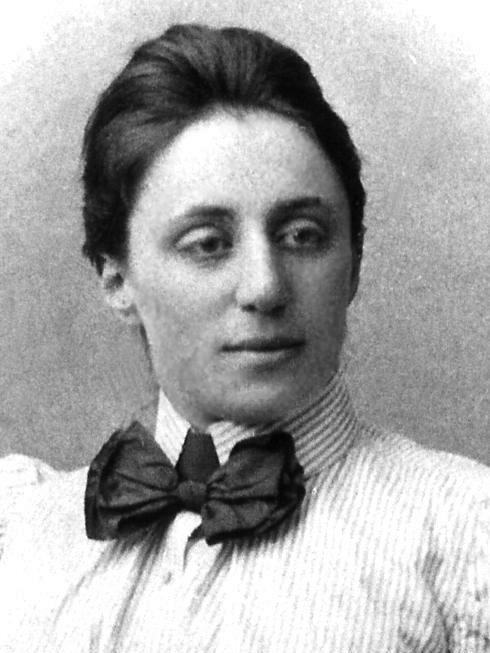
\includegraphics[scale=0.5]{emmy-noether.png} 
\caption{Emmy Noether. Photo Credit: Wikimedia Commons.} 
\end{figure}
Emmy Noether was born on Erlangen, Germany on March 23, 1882,
to an upper-middle class scholarly family. Hailed as the "mother of modern
algebra," and despite the barriers to women's
education that were prevalent at the time, Noether was, and remains to be,
a well-respected scholar in both mathematics and physics. Young girls at the
time were meant to be educated in arts and were not allowed to attend
college preperatory schools. After auditing classes at the University
of G\"{o}ttingen and the University of Erlangen, she finally enrolled at Erlangen
in 1904 when their policy was updated to allow female students. She recieved
a Ph.D. in mathematics in 1907.



In 1933, due to the rise of anti-Semitic government policy in Germany, Emmy
was let go from her position at G\"{o}ttingen. Because of her Jewish heritage
and her leftist political stance, she was forced to leave Germany. Luckily, Noether
 was able to emigrate
to the United States for a temporary position at Bryn Mawr, Pennsylvania. During
her time there she also lectured at Princeton, although she found the univeristy to
be unwelcoming to women \citep[81]{dick1981}. In 1935 Noether underwent an
operation to remove a uterine tumour. She passed away due to an infection as 
a result of the surgery, and was buried at Bryn Mawr.



\end{document}